\documentclass[journal,11pt]{IEEEtran}
\ifCLASSINFOpdf \else \fi

\usepackage{graphicx}

% *** MATH PACKAGES ***
\usepackage[cmex10]{amsmath}
\usepackage{amssymb}

\usepackage{tikz}
\usepackage{pgfplots}

%
% *** Algorithm PACKAGES ***
\usepackage{algorithmic}
%
% *** ALIGNMENT PACKAGES ***
\usepackage{array}
%
% *** SUBFIGURE PACKAGES ***
\ifCLASSOPTIONcompsoc
 \usepackage[caption=false,font=normalsize,labelfont=sf,textfont=sf]{subfig}
\else
 \usepackage[caption=false,font=footnotesize]{subfig}
\fi
%
% *** PDF, URL AND HYPERLINK PACKAGES ***
\usepackage{url}
%
% correct bad hyphenation here
\hyphenation{op-tical net-works semi-conduc-tor}
\usepackage[noadjust]{cite}

\begin{document}

\title{Blockchain Multiparty Computation Markets at Scale}

\author{{Charles~Noyes}% <-this % stops a space
\thanks{C. Noyes is with Villa Park High School, Villa Park,
CA, 92861 USA e-mail: cnoyes@usc.edu.}% <-this % stops a space
\thanks{Manuscript received December 00, 0000}}

% The paper headers
\markboth{IEEE Transactions on XXXXX,~Vol.~0, No.~0, December~0}%
{Shell \MakeLowercase{\textit{et al.}}: Bare Demo of IEEEtran.cls for Journals}




% make the title area
\maketitle

% As a general rule, do not put math, special symbols or s
% in the abstract or keywords.
\begin{abstract}
We explore ways of allowing for the offloading of computationally rigorous tasks from devices with slow logical processors onto a network of anonymous peer-processors. Recent advances in secret sharing schemes, decentralized consensus mechanisms, and multiparty computation (MPC) protocols are combined to create a P2P MPC market. Unlike other computational "clouds", ours is able to generically compute any arithmetic circuit, providing a viable platform for processing on the semantic web. Finally, we show that such a system works in a hostile environment, that it scales well, and that it adapts very easily to any future advances in the complexity theoretic cryptography used. Specifically, we show that the feasibility of our system can only improve, and is historically guaranteed to do so.
\end{abstract}

% \begin{IEEEkeywords}
% IEEEtran, journal, \LaTeX, paper, template.
% \end{IEEEkeywords}

\IEEEpeerreviewmaketitle

\section{Introduction}
\IEEEPARstart{C}{urrently,} computation is done locally in nearly all cases. Sans dedicated high-performance distributed computation scenarios, on-device logical processors are used to do all necessary computation. There are a number reasons for this. Foremost, there is simply a lack of an alternative. While services like Google's Cloud, Microsoft's Azure, Amazon Webservices, etc. allow for scalable distributed computation in specific and perfectly-predefined scenarios, no platform for generic "cloud" evaluation of arithmetic circuits exists.

\par Consider the implications of such a system; it would be able to sate small, networked devices' needs for high-performance processing power, allowing individual devices to tackle problems far larger than they are currently capable of. The rate of iterative processor upgrades would greatly slowed, as the expansion of device capability would no longer be conflated with corresponding logical processor updates. In effect, it would allow the burgeoning Internet of Things (IoT) to grow at a much faster rate, with a lower barrier to market entry.

\par The main non-trivial problems that must be solved here are assurances of security and scalability of the system. For the former, because we envision a system that is simply a cryptoeconomically-driven protocol, and not a service dependent on a centralized authority, a scheme for distributed consensus and trustless auditing must be designed. Neither problem is particularly hard, at least not seemingly insurmountably so, on its own, but when working in tandem, a behemoth results; scalability is trivial when security is compromised, and vice versa. However, when we wish to maintain verifiable security and absolute privacy, scalability becomes elusive. Homomorphic and Somewhat-Homomorphic Encryption (HE and SHE) schemes do not lend themselves to speed, but to security. Likewise, fast scheduling algorithms break down in the presence of adversaries - for example, one investigated SHE scheme, Shamir's~\cite{Shamir1979HowSecret}, can only guarantee correctness of multiplicative operations with $\mathcal{O}(n^2)$ communications, because of the degree reduction step of the process. 


\section{Related Work}
\par The interaction of the above two requirements is where other approaches break down. One of the better known "Semantic Web" projects is Ethereum\cite{Wood2014Ethereum:Ledger}, an offshoot of Bitcoin~\cite{Nakamoto2008Bitcoin:System} that allows for decentralized code execution - the caveat being that intensive work is economically and computationally infeasible, at best. The reason for this is a global execution scheme; consensus is held through the execution of circuits by all participants in the network, instead of having global verification of a zero knowledge proof. 

\par Perhaps the most closely related project, MIT's Enigma~\cite{Zyskind2015}, actually addresses this problem, but still falls a few steps short in its vision. While they draw on very similar ideas as we do here, they are taken only to the extent of providing a platform for private decentralized "analysis" - the reasoning being that truly fast decentralized \textit{computation} is a much more ambitious goal. We present a set of securely decentralizable schemes that allow for that computation at scale, such that the power of our network is not bounded by such restrictive constraints.

\par The most important prerequisite to an understanding of our work is knowledge of the workings of Bitcoin and its derivative 'blockchain' architectures. To summarize the body of very recent work surrounding them, consider a blockchain to be a canonically unchangeable decentralized ledger. Usually, both to give the work expended by the miners of the chain value and as its main purpose, a blockchain is used to store value digitally. However, the uses are far greater.

\section{Our Approach}
\par In order to accomplish the goals set forth we have constructed the cryptographic equivalent of a Panopticon. Our system enables privacy of data, speed of execution (relative to contemporary methodologies), and irreversibility of results. The first and last points lend themselves necessarily to security.


\subsection{Secure Data Distribution}
\begin{figure}
  \centering
  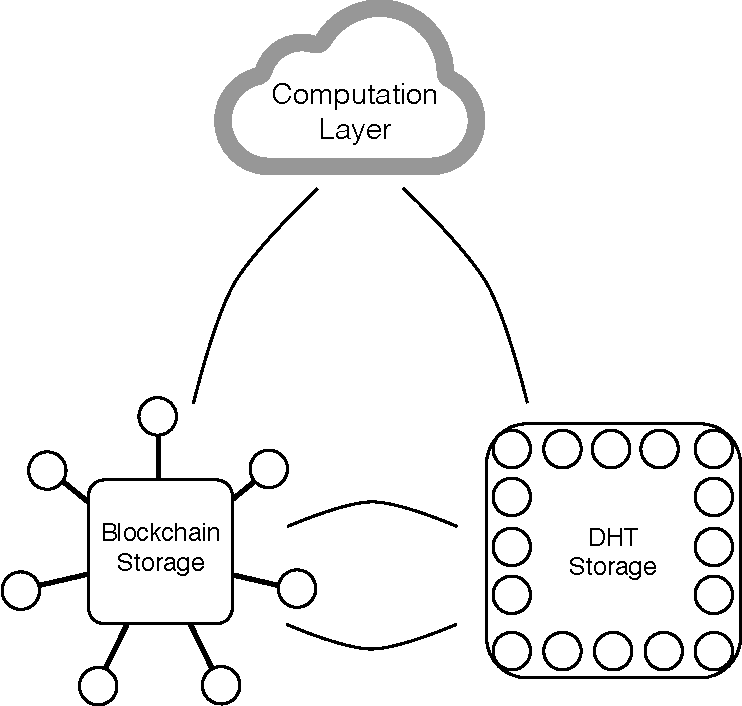
\includegraphics[width=2.5in]{figs/storageInteractions}
  \caption{Storage Interactions}
  \label{storage}
\end{figure}
\par One of the core tenants of our system is the availability of user data to computational entities. We accomplish this with a distributed hash table (DHT) that is hosted by our computational entities, to store the encrypted user data, and a public ledger (commonly known as a blockchain), which stores the data used to validate the machinations of the network.

\par Because of the way that blockchains are shared (all nodes must hold all data at all times), they do not lend themselves to large data networks. Because of this, only small proofs, like cryptographic commitments and keys, are stored. Additionally, generic currency features are supported, as it is easier to integrate into a new cryptocurrency than to adapt to an existing blockchain.

\par Conversely, distributed hash tables are very good at distributing large amounts of data to many different nodes. The size of the network is thus not limited by the total amount of data stored, as the amount that each node must store scales inversely with the number of participants.

\subsection{Secure Contract Execution}
\par Our contract execution scheme is described in greater technical detail in the following sections. To give an overview, computation is done in a modified decentralized fashion. Small proofs included on the blockchain are used to ensure correctness of off-chain computation, and Ethereum-like smart contracts are able to be included on the blockchain proper. These smart contracts are Turing-complete but have a cost associated with each computational step in their execution. In addition, they continue to live on the blockchain until they are removed.

\par The meat of our system, the off-chain computational contracts, are transient and only their proofs are included on the blockchain. They are able to access both on-blockchain and DHT storage, but are unable to modify the on-blockchain storage associated with smart contracts.

\section{Computation}
\par Here we describe our computational model in exact detail. To begin, a brief overview of publicly verifiable secure multiparty computation (sMPC) is needed. Note that our actual computational model is derived from Enigma's~\cite{Zyskind2015}. We make use of the same computational paradigms, but our network model is directed much differently. 

\subsection{Private Computation}
\par Two-party computations protocols were pioneered by Yao in~\cite{Yao1982ProtocolsComputations}. Yao proposed the millionaire problem, in which two individuals wish to compare wealth without revealing exact sums. This problem has since been generalized for \textit{n-party} cases, but because of the composition of elementary circuits a solution to the millionaire problem (in the n-party case) is a solution to sMPC. Yao proposed the use of garbled circuits~\cite{Huang2011FasterCircuits.}, but they do not scale. Secret sharing, based on threshold cryptography, is a much more common and scalable solution.

\par Shamir introduced the idea of secret sharing using polynomial secrets in~\cite{Shamir1979HowSecret}. These are known as threshold cryptosystems, as they are defined by a ($(t+1,n)$)-\textit{threshold}, where $n$ is the number of participants and $t+1$ is the minimum number of parties needed to decrypt a secret. $t$ (or any of its subsets) cannot learn anything about the secret. \textit{Shamir's secret sharing scheme} (\textit{SSS}) is an example of a scheme which uses polynomial interpolation to allow for security under a finite field. To share a secret $k$, a random polynomial $P(x)$ of degree $t$ is selected 
\begin{gather}
P(x) = a_{t}x^t + ... a_0 \\
a_0 = s
\end{gather}

\par The shares are then given by evaluating $P(x)$ over $[1,n]$ and distributing accordingly. Then, given any $t+1$ shares, $P(x)$ is able to be determined via Lagrange interpolation and our secret given by $k = P(0)$. Multiplication by scalars and additive homomorphism are supported locally simply by direct operation. Given secrets $s_1,s_2$ and a scalar $q$,

\begin{gather}
q \times s = Interpolate(\{q[s]_i\}\substack{i=t+1\\i=0} \\
s_1 + s_2 = Interpolate(\{[s_1]_i + [s_2]_i]\})\substack{i=t+1\\i=0}.
\end{gather}

\par Multiplication is significantly harder. While the addition of two secrets of degree $t$ does not change the degree of the resulting secret, the multiplication of those secrets will result in a polynomial of degree $2t$. The degree reduction step requires $\mathcal{O}(n^2)$ communication. 

\par So, we are left with a cryptosystem that allows for the computation of arbitrary circuits, as additive and multiplicative operations form any boolean circuit, on completely private data.

\par Note that the referenced '$Interpolate$' is simply the operation
\begin{gather} 
P_i(x) = \prod_{j\neq\,i}^{t+1} \frac{x - x_j}{x_i - x_j},
\end{gather}
a general Lagrangian interpolation. 

\subsection{Speedy Computation}
\par The above is excellent for securely private computation -- however, there are many cases in which perfect privacy is not a concern, or in which a lack of privacy is overshadowed by a want for speedier computation. We are able to satisfy this need with a simpler protocol, that makes use of Ethereum's Turing-completeness. The basic scheme is very simple: data is committed to the DHT in an encrypted format, a request is appended to the blockchain, a commitment to computation as well as a deposit is made by a computational entity, the requester puts up an agreed-upon deposit (perhaps influenced by prior actions on the same public key), and the computational entity begins its work after receiving a decryption key for the data to be computed on.
\begin{figure}
  \centering
  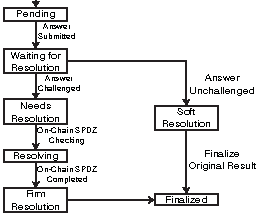
\includegraphics[width=2.5in]{figs/flowchart}
  \caption{Secure Computation Validation}
  \label{validation}
\end{figure}
\par Before getting into the details of result verification, there are a few interesting features of this paradigm that are not present in the securely-private model enumerated in the previous section. For example, the computation does not have to be done in predefined "rounds," the input data can be formatted in any way, and the language used can be far more expansive. Of course, the most obvious difference is that all computation is done (from the perspective of the submitted) entirely locally. There are no share-resharing or secret reconstructions steps, and the computation does not have to be fitted into a branched arithmetic circuit. Note that while the computation appears to be local, it is really just airgapped from the network at large, as a computational entity is free to do it on a locally distributed system (assuming they are able to retain correct proofs).

\par Finally, after computation is complete and the result is committed to and submitted by the computing entity, result validation can begin. The result is codified onto the blockchain, so it is always the first entity to finish that is awarded the bounty if no conflicting answers are submitted. However, if another computing entity is willing to back their stake on the assumption that the original result was incorrect, and the verification procedure outlined in Fig.~d\ref{validation} supports this, they are awarded both the deposits of all malicious/incorrect entities and the original bounty. Thus, it is obviously, in a game-theoretic sense, in the best interest of computational entities to be honest.

\subsection{Verifiability}

\par Ethereum is able to validate SPDZ proofs~\cite{Laud2014VerifiableMajority} on a challenge. This is one of the core innovations introduced by this project. SPDZ are, essentially, computational proofs that are significantly easier to create and audit than any other existing system~\cite{BaumEfficientAbort}. Some notation is needed to properly define the protocol. Let $n$ be the number of players and $\mathbb{F}_q$ the finite field we do computations on. Each player $P_i$ has a share $a_i \in \mathbb{F}_q$ of a shared secret value $a = a_1 + ... + a_n$. This $a$ is known as the fixed MAC key. Each player $P_i$ also has a secret key $B_1$. 

\par $[x] x \in \mathbb{F}_q$ is $\big[{}\cdot{}\big]$-shared if $P_i$ holds a tuple $(x_i,y(x)_i)$ where $x_i$ is an additive secret sharing of $x$, i.e. $x = x_1 + ... + x_n$, and $y(x)_i)$ is an additive secret sharing of $y(x) = ax$.

\par $[x] x \in \mathbb{F}_q$ is $\big[{}\big[{}\cdot{}\big]{}\big]$-shared if $P_i$ holds a tuple $(x_i,y(x)_i)$ where $x_i$ is an additive secret sharing of $x$ and $\forall{}k \in [1,n]:y_k(x)_i$ is an additive secret sharing of $y_k(x) = B_kx$.

\par Next, there is both an online and offline phase. The offline phase consists of the construction of raw material to be passed to the online phase. Using~\cite{Lindell2015EfficientSPDZ}, we are able to  reuse fixed MAC keys, reducing the computational complexity of the initial calculations significantly. Additionally, we use the results from~\cite{BaumBetterComputation} to make this scheme publicly auditable. Our blockchain acts as the 'bulletin board' described in the paper, as each step's proofs are pegged to the blockchain. This also ensure we are able to be sure (in the securely-private model) of which actor was malicious. 

\par Lastly, we have need of a public auditor. This is a massive problem for a decentralized sMPC system that uses SPDZ proofs; however, we have the perfect system to do these audits. Ethereum's blockchain is Turing-complete and the auditing of computations involves only very simple operations. Thus, we are given the last key to the game-theoretic puzzle behind this project.


\section{Results}
\begin{figure}
  \centering
  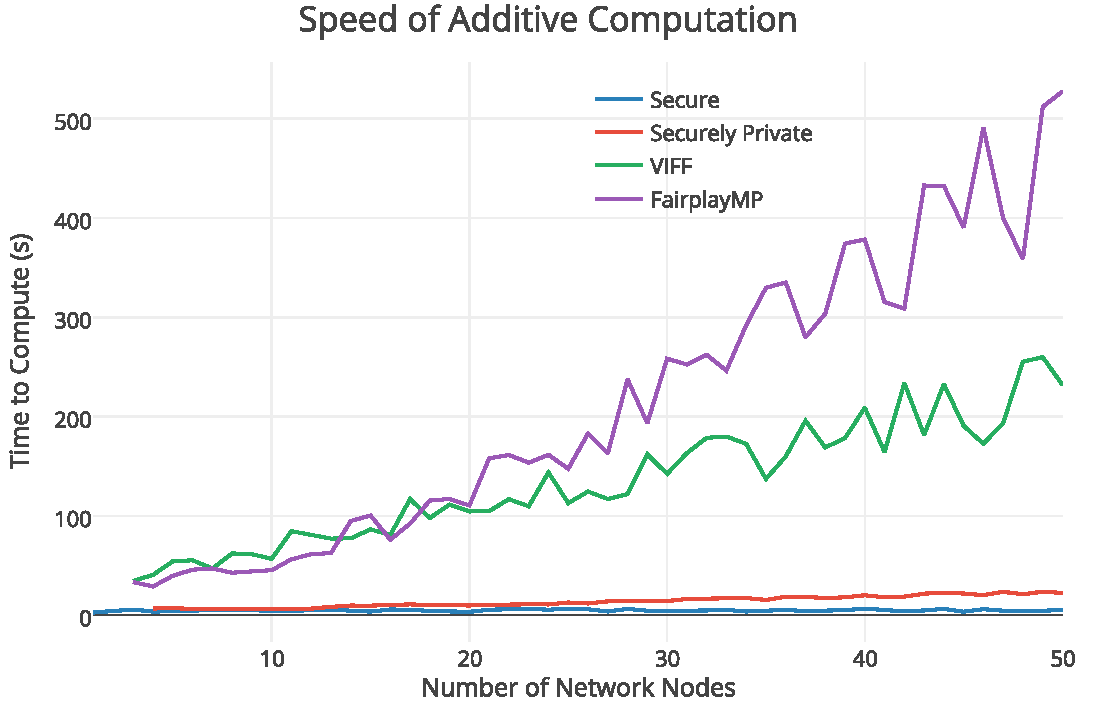
\includegraphics[width=3.5in]{speedAdd}
  \caption{}
  \label{speedAdd}
\end{figure}
\par We compared Pandora (both the secure and securely private models) to two other open source implementations of sMPC protocols. First, FairplayMP~\cite{Ben-David2008FairplayMP:Computation} is an academic project by the Hebrew University of Jerusalem that uses garbled Boolean circuits to securely compute functions on secret data in the n-party case. VIFF~\cite{Geisler2007VIFF:Framework} is an open source sMPC project that uses arithmetic circuit evaluation, without a public board (in our case the blockchain), and a variety of different optimization techniques. Neither is optimized for speed or scalability, but they are in fact the only two public sMPC projects we could find.

\par For additive computations, we calculated very large terms of the Fibonacci sequence. This tested our system’s ability to deal with large numbers, stateful computational rounds, and basic scalar multiplication and summation. Both of our paradigms outperformed FairplayMP and VIFF by large margins; our secure model was between 2,000\% and 4,000\% faster than other test projects (5 sigma confidence). Our securely private model was marginally (~2.8x, 5 sigma confidence) slower than our secure model, however it was still significantly faster than FairplayMP and VIFF (950\% and 1600\%, respectively, at six sigma confidence).
\begin{figure}
  \centering
  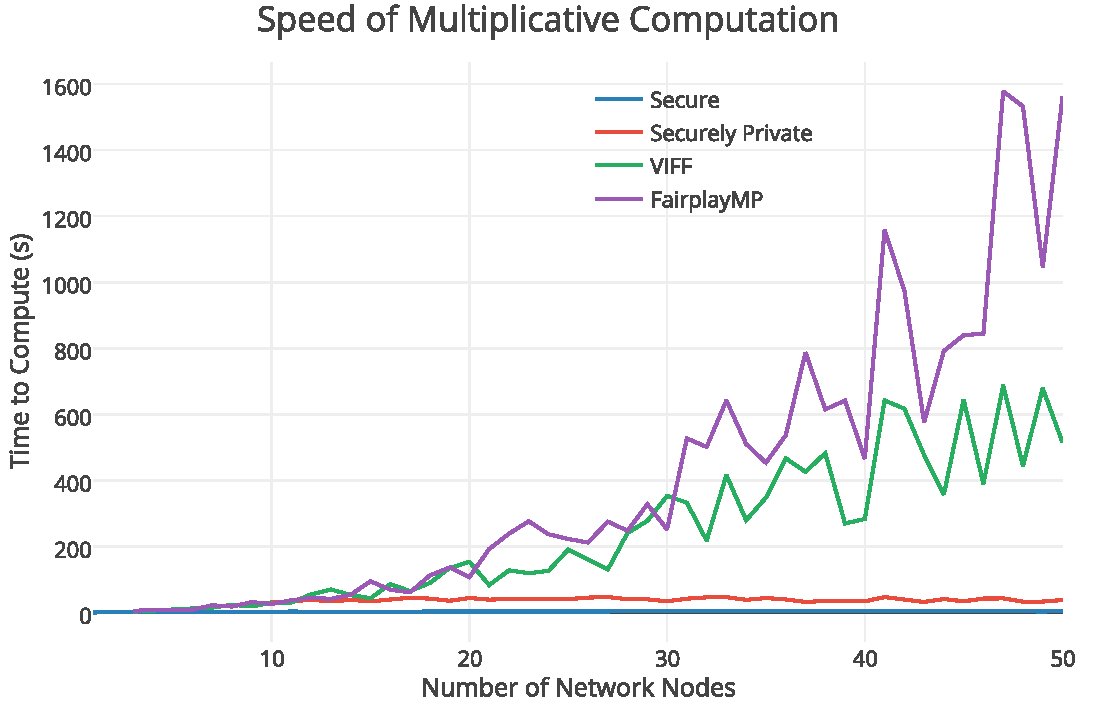
\includegraphics[width=3.5in]{speedMult}
  \caption{}
  \label{speedMult}
\end{figure}
\par Our securely private model is most comparable to FairplayMP and VIFF, because both utilize advance homomorphic cryptosystems. We believe we saw such favorable results, specifically for the additive step of our securely private model, because our system doesn’t require verification at each computational round. This trait also introduces per-round network communication complexity $\mathcal{O}(n^2)$, whereas our system requires no communication whatsoever to maintain security.

\par For multiplicative computations, we calculated very large terms of the irrational number Pi via Chudnovsky’s algorithm. This tested our system’s ability to deal with extremely long decimal values, stateless computational rounds, and homomorphic multiplication of encrypted shares (for the securely private model. Our security-only model was, on average, 950\% faster than the securely private model (5 sigma confidence), 6,300\% faster than VIFF (5 sigma confidence), and 10,700\% faster than FairplayMP (5 sigma confidence. Our securely private model was also faster than both other solutions, by smaller but similar margins. What is really interesting, however, is how our securely private model scales so incredibly well compared to both VIFF and FairplayMP. The reason for this is described in our conclusion.

\par Lastly, we showed that 

% \begin{figure}[!t]
% \centering
% \hspace*{-1.5cm} 
% \begin{tikzpicture}
% \begin{axis}[
%     compat=newest, %Better label placement
%     ybar = 0.6,
%     width=0.6\textwidth,
%     ymin=0,
%     bar width=6pt,
%     title={End-to-End Speed vs. Industry Solutions},
%     legend style={at={(0.5,-0.225)},
%     anchor=north,legend columns=0},
%     ylabel={Overhead (\%) },
%     x tick label style={rotate=45, anchor=east,font=\small,text width=1.7cm,align=center},
%     xticklabels={Securely Private, Secure, Hadoop}
%     xtick={1,2,3},
%     axis lines*=left,
%     ytick style={draw=none},
%     cycle list={
%         {fill=black!80,draw=black!80},
%         {fill=black!60,draw=black!60},
%         {fill=black!40,draw=black!40}
%     },
%     axis on top,
%     major grid style=white,
%     ymajorgrids,
%     legend style={draw=none,/tikz/every even column/.append style={column sep=0.5cm}}
%  \addplot 
% 	coordinates {(1, 2.3)};
%  \addplot 
% 	coordinates {(2, 1.2)};    
%  \addplot 
% 	coordinates {(3, 1.0)};
% ]
% \legend{Best,Average,Worst}
% \end{axis}
% \end{tikzpicture}
% \caption{Throughput Graph}
% \label{graph_through}
% \end{figure}
\par Lastly, we tested our system's speed in relation to the Hadoop scheduler. Essentially, instead of distributing normal computational tasks, we had it distribute sMPC-driven computations. The overhead on our fastest model was minimal ($20\%$), while the overhead on our securely private model was managable but significant ($110\%$). These are our most recent findings.


\section{Conclusion}
\par My findings showed that the implementation of our proposed design exceeded expectations in all areas of performance. Through the use of state-of-the-art advances in cryptography, distributed consensus systems, and game-theoretic protocols for secure computation, we have managed to devise a realistic system for fast, secure, and incentivized secure multiparty computation. 

\par Our original design was left mostly intact. The main revision was the addition of a feed-forward execution loop for the pruning of nodes in individual securely private computational rounds. Essentially, after every round the tree of nodes participating is pruned by some predefined metric, such that only the fastest (both computationally and by ping) are left. Additionally, we are working on a pre-computation segmenting algorithm.

\par With the exception of the above problem (and solution), most problems encountered had to do with the dually computational and game-theoretic nature of this project. As opposed to systems like FairplayMP and VIFF, we must constantly take into account that there is a very real incentive (beyond mischief) for an attacker to try to co-opt or subvert our network. Thus, protocols like the aforementioned challenge-deposit are required. Small details like those are scattered throughout the project, in far, far, larger numbers than we could present here.

\par As for Pandora’s implications, it stands to completely revolutionize the internet as we know it. Although Pandora may be a stepping stone, it is the first of its kind. “Web 3.0” is commonly defined as “connective intelligence” – it will connect concepts, data, applications, and, ultimately, people. That is a very pure distillation of what Pandora ultimately stands to do. It stands to globally unify the disparate computational systems that exist today. Leading industry figures are already moving in this direction of unification (see: Google et al.’s Open Compute), because it is simply beneficial for all involved.


\begin{IEEEbiographynophoto}{Charles Noyes}
is  attending Villa Park High School. He has participated in many high school science competition and enjoys doing research. He is interested in the ways that blockchains can be applied to areas other than digital currencies, and is currently looking for a research mentor.
\end{IEEEbiographynophoto}

\bibliographystyle{IEEEtran}
\bibliography{Mendeley.bib}
\end{document}